\documentclass[12pt]{article}
\usepackage[empty]{fullpage}
\usepackage{tikz}

\begin{document}
\section*{Project 1 - Tips}


\begin{enumerate}
\item How many spaces do you need to print in the each row before the first character of the diamond? You need to figure out the pattern of spaces and symbols to print in order to make the diamond.  

\begin{center}
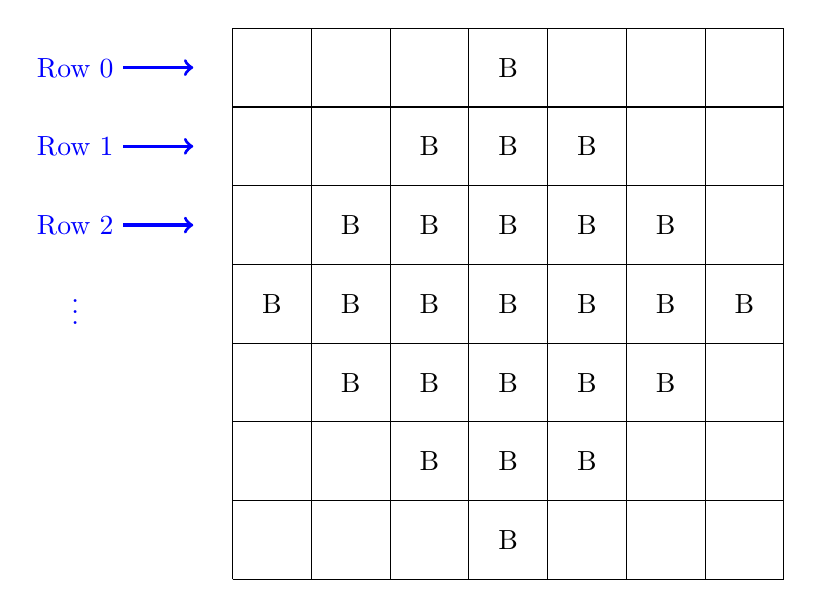
\begin{tikzpicture}
\draw(0,0) grid (7,7);
\draw(0.5,3.5) node {B};
\draw(1.5,3.5) node {B};
\draw(2.5,3.5) node {B};
\draw(3.5,3.5) node {B};
\draw(4.5,3.5) node {B};
\draw(5.5,3.5) node {B};
\draw(6.5,3.5) node {B};

\draw(1.5,4.5) node {B};
\draw(2.5,4.5) node {B};
\draw(3.5,4.5) node {B};
\draw(4.5,4.5) node {B};
\draw(5.5,4.5) node {B};

\draw(1.5,2.5) node {B};
\draw(2.5,2.5) node {B};
\draw(3.5,2.5) node {B};
\draw(4.5,2.5) node {B};
\draw(5.5,2.5) node {B};

\draw(2.5,1.5) node {B};
\draw(3.5,1.5) node {B};
\draw(4.5,1.5) node {B};

\draw(2.5,5.5) node {B};
\draw(3.5,5.5) node {B};
\draw(4.5,5.5) node {B};

\draw(3.5,6.5) node {B};
\draw(3.5,0.5) node {B};

\draw[very thick, blue,->] (-2,6.5) node[fill=white] {Row 0} -- (-0.5,6.5);
\draw[very thick, blue,->] (-2,5.5) node[fill=white] {Row 1} -- (-0.5,5.5);
\draw[very thick, blue,->] (-2,4.5) node[fill=white] {Row 2} -- (-0.5,4.5);
\draw[very thick, blue,->] (-2,3.5) node[fill=white] {$\vdots$};
\end{tikzpicture}

\end{center}

\item Don't forget you can combine strings by adding them: \verb|"try" + "this" + " out  !"|. You can also repeat a string if you multiply it by a number. 
\item To print a string without starting a new line, use the optional \verb|end = ""| argument:
\begin{center}
\verb|print("any string", end = "")|
\end{center}
\item Would it be helpful to use more than one for-loop for different parts of the diamond?
\item It helps to know the location of the middle row.  With $n$ rows, the middle row is $n$ divided by 2 rounded down (if you start counting from row 0). Use the \textbf{integer division} operator \verb|//| which divides integers and returns the answer without the  remainder.  Here are some examples:
\end{enumerate}

\begin{verbatim} 
      4 // 2 # returns 2
      7 // 2 # returns 3 
\end{verbatim}

\end{document}
